\chapter{Popis software}

Pojmem firmware je v této kapitole myšlen program, který je spuštěn v počítači, ke kterému je připojen reflektometr. Tento program slouží pro ovládání reflektometru, zobrazování změřených dat a kalibraci reflektometru. Kalibrace probíhá pomocí změření odezvy na tři mechanické kalibry. Software předpokládá kalibry \quotedblbase open\textquotedblleft, \quotedblbase short\textquotedblleft{} a \quotedblbase match\textquotedblleft{}.

Software je napsán v prostředí GNU Octave a určen pro operační systém GNU/Linux. S menšími úpravami by mělo být možné tento software provozovat i pod operačním systémem Windows. Prostředí Octave je z převážné části kompatibilní s programovacím jazykem MATLAB, v lehce upravené podobě by mělo být možné ovládací program spustit i  v prostředí MATLAB. Prostředí Octave bylo zvoleno, protože jde o jazyk určený pro matematické úlohy, podobně jako MATLAB, ovšem je šířeno zdarma pod licencí GNU GPL, k obsluze reflektometru tedy není třeba pořizovat nákladnou licenci na prostředí MATLAB. Další výhodou je, že Octave je multiplatformní, a není tedy vázáno jen na běžné počítače, ale je možné jej provozovat i na levných jednodeskových počítačích, např. na Raspberry Pi.

\section{Ovládání software}

Nejprve software testuje dostupnost sériových portů podle obr. \ref{serial_probe}. Tento problém může na operačním systému GNU/Linux nastat v příadě, kdy uživatel, který prostředí Octave spouští, nemá dostatečná práva na přístup k sériovým portům. Druhou možností, kdy k této chybě může dojít, je v případě, kdy je Octave spouštěno z kontejneru Flatpak bez povolení k přístupu k hardware. V případě operačního systému Windows může být příčinou chyby buď nedostatečné oprávnění uživatele nebo otevření sériového portu jiným programem, protože oproti operačnímu systému GNU/Linux neumožňuje otevřít sériový port ve více programech najednou.
\begin{figure}[H]
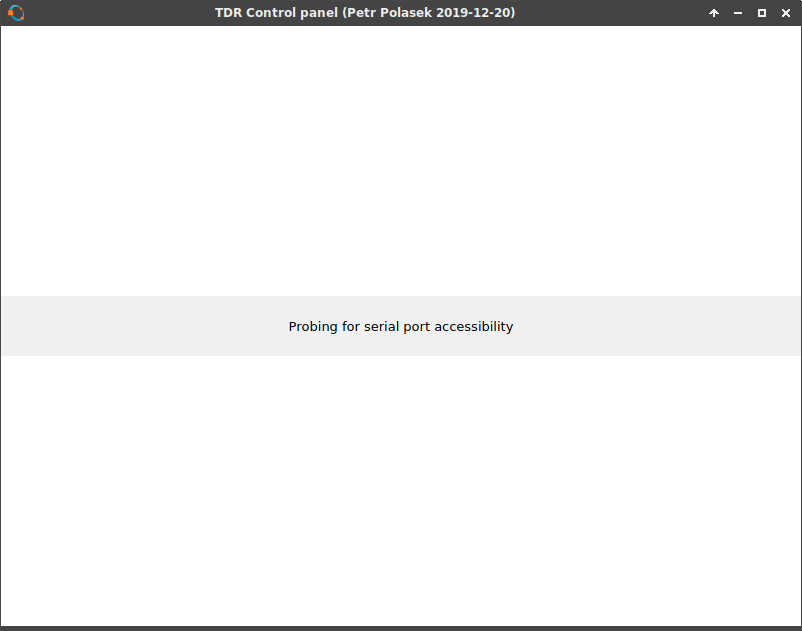
\includegraphics[width=\textwidth,keepaspectratio]{images/gui/serial_probe.png}\caption{Test dostupnosti sériových portů.}\label{serial_probe}
\end{figure}	

V případě, že dojde k problému s přístupem k sériovému portu, je o této skutečnosti uživatel nformován včetně nápovědy, co je možné v tomto případě dělat podle obr. \ref{serial_port_unsupported}. Uveden je příklad opravy spouštěcího příkazu pro kontejnery Flatpak.
\begin{figure}[H]
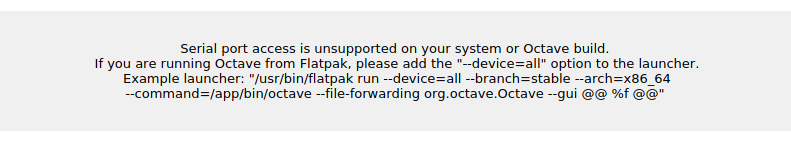
\includegraphics[width=\textwidth,keepaspectratio]{images/gui/serial_port_unsupported_cut.png}\caption{Chybové hlášení o nedostupnosti sériových portů, oříznuto.}\label{serial_port_unsupported}
\end{figure}	

V případě, že je přístup k sériovým portům povolen, začne program vyhledávat virtuální sériové porty připojené přes USB, přičemž zobrazí hlášení jako na obr. \ref{serial_port_lookup}. Ty se v prostředí GNU/Linux jmenují \verb"/dev/ttyUSB*". 
\begin{figure}[H]
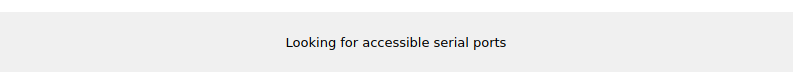
\includegraphics[width=\textwidth,keepaspectratio]{images/gui/serial_port_lookup_cut.png}\caption{Hledání sériových portů.}\label{serial_port_lookup}
\end{figure}

Pokud není nalezen žádný virtuální sériový port, je zobrazeno hlášení na obrázku \ref{serial_no_port_available}, které vyzývá uživatele k připojení reflektometru. Pokud je vhodný port nalezen, zobrazí se hlášení z obrázku \ref{serial_port_found}.
\begin{figure}[H]
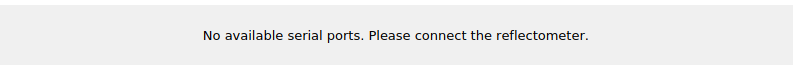
\includegraphics[width=\textwidth,keepaspectratio]{images/gui/serial_no_port_available_cut.png}\caption{Hlášení v případě, kdy není připojen žádný virtuální sériový port.}\label{serial_no_port_available}
\end{figure}

\begin{figure}[H]
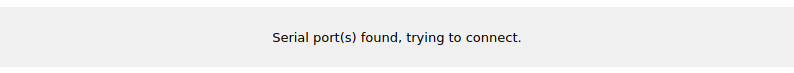
\includegraphics[width=\textwidth,keepaspectratio]{images/gui/serial_port_found_cut.png}\caption{Hlášení v případě, kdy je nalezen vhodný virtuální sériový port.}\label{serial_port_found}
\end{figure}

Software následně nalezený port otestuje tak, že na něj pošle zprávu \verb"DEV?", na kterou očekává odpověď. V případě, že je součástí odpovědí text \verb"TDR5351_CORE", software použije tento port pro komunikaci s reflektometrem. Plná identifikace zařízení obsahuje ještě informaci o datu a času kompilace firmware, tento identifikátor je vidět na obr. \ref{serial_device_found}. Zařízení je následně poslán příkaz \verb"REM!", kterým je zařízení informováno o požadavku na dálkové ovládání. Software očekává potvrzení ve formě zprávy \verb"REM.", načež se spustí vlastní rozhraní pro ovládání reflektometru. Celý úspěšný proces potvrzování je ještě indikován zprávou na obr. \ref{serial_accepted}.
\begin{figure}[H]
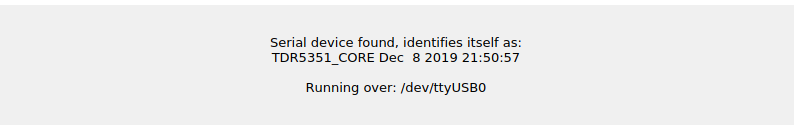
\includegraphics[width=\textwidth,keepaspectratio]{images/gui/serial_device_found_cut.png}\caption{Hlášení v případě, kdy je nalezen vhodný virtuální sériový port.}\label{serial_device_found}
\end{figure}

\begin{figure}[H]
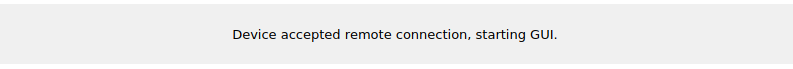
\includegraphics[width=\textwidth,keepaspectratio]{images/gui/serial_accepted_cut.png}\caption{Informace o úpěšném potvrzení vzdáleného přístupu.}\label{serial_accepted}
\end{figure}

Po připojení k reflektometru se zobrazí ovládací rozhraní, které je vidět na obr. \ref{gui_edge_wait}. V tuto chvíli čeká reflektometr na odpojení všech zařízení od měřicího portu a potvrzení uživatelem. To je možné udělat jak barevně zvýrazněným tlačítkem CONTINUE, tak stiskem tlačítka na reflektometru. V případě odpojení ovládacího programu je možné program znovu spustit, přičemž reflektometr tato událost nijak nezasáhne - není potřeba znovu provádět autokalibrace, ani se nepřeruší měření. Grafické rozhraní je možné k reflektometru připojit kdykoli, není potřeba jej spustit při zapínání reflektometru.
\begin{figure}[htbp]
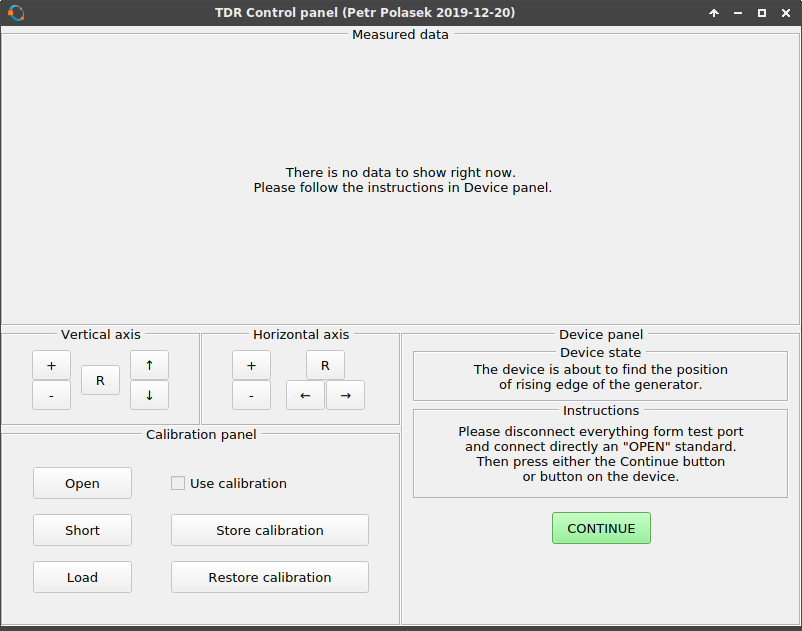
\includegraphics[width=\textwidth,keepaspectratio]{images/gui/edge_wait.png}\caption{Grafické rozhraní, čekání na zásahu uživatele - autokalibrace napěťových úrovní, úrovně šumu a hrubé pozice budicího pulzu.}\label{gui_edge_wait}
\end{figure}

Grafické rozhraní postupně uživatele provází autokalibrací, vždy poskytuje informace o aktuálním probíhajícím kroku. Zároveň informuje uživatele srozumitelnou formou o tom, co se od něj očekává. Veškerá tlačítka se podle aktuálního stavu automaticky uzamykají a odemykají, případně podbarvují nebo mizí tak, aby uživatel nemohl provést neočekávaný požadavek, který by v dané chvíli buď nedával smysl, případně uživatele mátl.

V okamžiku, kdy jsou provedeny všechny autokalibrační procesy, je uživateli předloženo rozhraní podle obr. \ref{dut_ready}. Objevily se nové ovládací prvky, tlačítko RUN a posuvník pro nastavení počtu průměrování. Uživatel může nastavit pomocí posuvníku požadovaný počet průměrování. Program automaticky nastaví na posuvníku počet průměrování, který je dle odhadu šumové úrovně ideální, nicméně uživatel může toto nastavení dle svých potřeb změnit v rozsahu \SIrange{1}{64}{}. 
\begin{figure}[htbp]
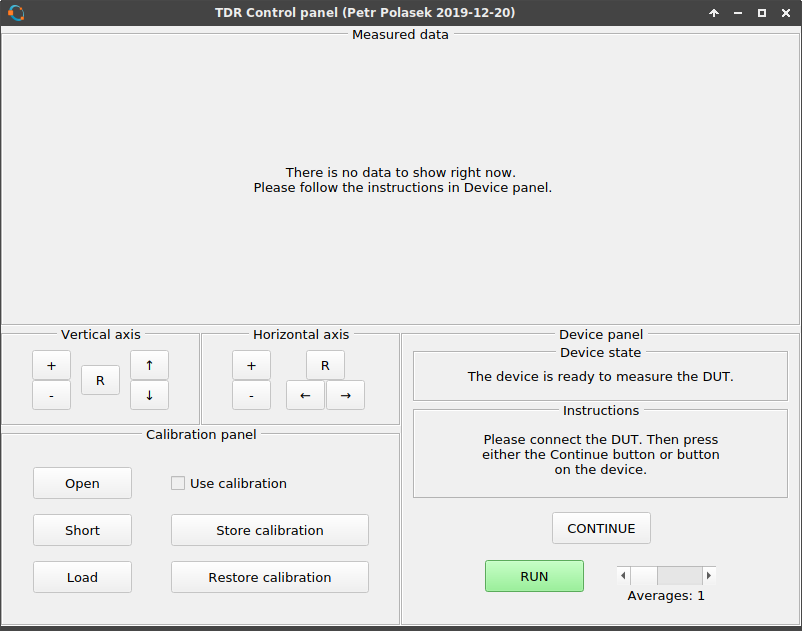
\includegraphics[width=\textwidth,keepaspectratio]{images/gui/dut_ready.png}\caption{Grafické rozhraní, zařízení je připraveno na měření.}\label{dut_ready}
\end{figure}

Jakmile software obdrží první měřená data, zobrazí je v grafu jako na obr. \ref{measured_data}. Poté se odemknou ovládací prvky a s grafem je možné manipulovat. Graf je možné horizontálně i vertikálně zvětšovat i posouvat. V případě nastavení mimo změřená data je možné osy resetovat do původního stavu.
\begin{figure}[htbp]
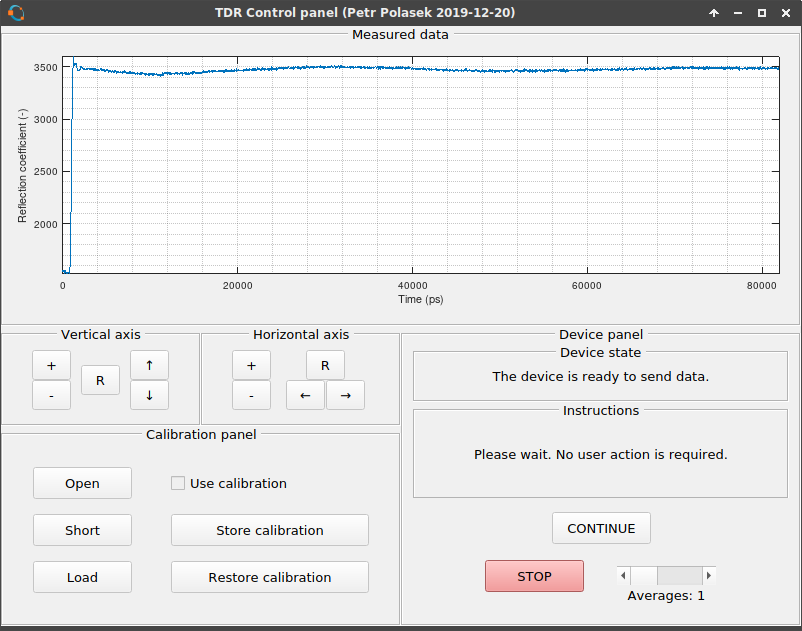
\includegraphics[width=\textwidth,keepaspectratio]{images/gui/measured_data.png}\caption{Probíhající měření s aktuálními změřenými daty.}\label{measured_data}
\end{figure}

Ve stavu, kdy již bylo provedeno měření a reflektometr je připraven k dalšímu měření, je možné stisknout tlačítka na kalibračním panelu. Stiskem tlačítek \quotedblbase Open\textquotedblleft, \quotedblbase Short\textquotedblleft{} nebo \quotedblbase Load\textquotedblleft{} se uloží kalibrační data pro daný mechanický kalibr, který byl předtím takto změřen. Kalibrační data je možné odstranit opětovným stiskem tlačítka. Je-li tlačítko vybraveno žlutě, má software pro daný kalibr již uložena kalibrační data. Od okamžiku, kdy se uloží kalibrační data pro standard \quotedblbase load\textquotedblleft , je pro zobrazování změřených dat použita jednoduchá základní kalibrace, která spočívá v tom, že od měřených dat je odečten průběh dpovídající kalibru \quotedblbase load\textquotedblleft . Tato částečná kalibrace se dá vypnout pouze tak, že se odstraní data pro kalibr \quotedblbase load\textquotedblleft , protože bylo vypozorováno, že aplikace této základní kalibrace výrazně potlačuje stejnosměrný posun měřených dat a zvlnění průběhu. Toto zvlnění je opakovatelné a prakticky neměnné, proto je možné jej takto jednoduše potlačit. 